% Created 2021-06-08 二 14:40
% Intended LaTeX compiler: pdflatex
\documentclass[11pt]{article}
\usepackage[utf8]{inputenc}
\usepackage[T1]{fontenc}
\usepackage{graphicx}
\usepackage{grffile}
\usepackage{longtable}
\usepackage{wrapfig}
\usepackage{rotating}
\usepackage[normalem]{ulem}
\usepackage{amsmath}
\usepackage{textcomp}
\usepackage{amssymb}
\usepackage{capt-of}
\usepackage{hyperref}
%%%%%%%%%%%%%%%%%%%%%%%%%%%%%%%%%%%%%%
%% TIPS                                 %%
%%%%%%%%%%%%%%%%%%%%%%%%%%%%%%%%%%%%%%
% \substack{a\\b} for multiple lines text

\usepackage[utf8]{inputenc}

\usepackage[B1,T1]{fontenc}

% pdfplots will load xolor automatically without option
\usepackage[dvipsnames]{xcolor}
%%%%%%%%%%%%%%%%%%%%%%%%%%%%%%%%%%%%%%%
%% MATH related pacakge                  %%
%%%%%%%%%%%%%%%%%%%%%%%%%%%%%%%%%%%%%%%
% \usepackage{amsmath} mathtools loads the amsmath
\usepackage{amsmath}
\usepackage{mathtools}


\usepackage{amsthm}
\usepackage{amsbsy}

%\usepackage{commath}

\usepackage{amssymb}
\usepackage{mathrsfs}
%\usepackage{mathabx}
\usepackage{stmaryrd}
\usepackage{empheq}

%for \not\ll
\usepackage{centernot}

\usepackage{scalerel}
\usepackage{stackengine}
\usepackage{stackrel}

\usepackage{nicematrix}
\usepackage{tensor}
\usepackage{blkarray}
\usepackage{siunitx}
\usepackage[f]{esvect}

\usepackage{unicode-math}
\setmainfont{TeX Gyre Pagella}
% \setmathfont{STIX}
%\setmathfont{texgyrepagella-math.otf}
%\setmathfont{Libertinus Math}
\setmathfont{Latin Modern Math}

 
% \setmathfont[range={\smwhtdiamond,\enclosediamond,\varlrtriangle}]{Latin Modern Math}
 \setmathfont[range={\rightrightarrows,\twoheadrightarrow,\leftrightsquigarrow,\triangledown,\vartriangle}]{XITS Math}
 \setmathfont[range={\int,\setminus}]{Libertinus Math}
 \setmathfont[range={\mathalpha}]{TeX Gyre Pagella Math}
% unicode is not good at this!
%\let\nmodels\nvDash


%%%%%%%%%%%%%%%%%%%%%%%%%%%%%%%%%%%%%%%
%% TIKZ related packages                 %%
%%%%%%%%%%%%%%%%%%%%%%%%%%%%%%%%%%%%%%%

\usepackage{pgfplots}
\pgfplotsset{compat=1.15}
\usepackage{tikz}
\usepackage{tikz-cd}
\usepackage{tikz-qtree}

\usetikzlibrary{arrows,positioning,calc,fadings,decorations,matrix,decorations,shapes.misc}
%setting from geogebra
\definecolor{ccqqqq}{rgb}{0.8,0,0}


%%%%%%%%%%%%%%%%%%%%%%%%%%%%%%%%%%%%%%%
%% MISCLELLANEOUS packages               %%
%%%%%%%%%%%%%%%%%%%%%%%%%%%%%%%%%%%%%%%
\usepackage[most]{tcolorbox}
\usepackage{threeparttable}
\usepackage{tabularx}

\usepackage{enumitem}

% wrong with preview
\usepackage{subcaption}
\usepackage{caption}
% {\aunclfamily\Huge}
\usepackage{auncial}

\usepackage{float}

\usepackage{fancyhdr}

\usepackage{ifthen}
\usepackage{xargs}


\usepackage{imakeidx}
\usepackage{hyperref}
\usepackage{soul}


%\usepackage[xetex]{preview}
%%%%%%%%%%%%%%%%%%%%%%%%%%%%%%%%%%%%%%%
%% USEPACKAGES end                       %%
%%%%%%%%%%%%%%%%%%%%%%%%%%%%%%%%%%%%%%%

% \setlist{nosep}
% \numberwithin{equation}{subsection}
% \fancyhead{} % Clear the headers
% \renewcommand{\headrulewidth}{0pt} % Width of line at top of page
% \fancyhead[R]{\slshape\leftmark} % Mark right [R] of page with Chapter name [\leftmark]
% \pagestyle{fancy} % Set default style for all content pages (not TOC, etc)


% \newlength\shlength
% \newcommand\vect[2][0]{\setlength\shlength{#1pt}%
%   \stackengine{-5.6pt}{$#2$}{\smash{$\kern\shlength%
%     \stackengine{7.55pt}{$\mathchar"017E$}%
%       {\rule{\widthof{$#2$}}{.57pt}\kern.4pt}{O}{r}{F}{F}{L}\kern-\shlength$}}%
%       {O}{c}{F}{T}{S}}


\indexsetup{othercode=\small}
\makeindex[columns=2,options={-s /media/wu/file/stuuudy/notes/index_style.ist},intoc]
\makeatletter
\def\@idxitem{\par\hangindent 0pt}
\makeatother


%\newcounter{dummy} \numberwithin{dummy}{section}
\newtheorem{dummy}{dummy}[section]
\theoremstyle{definition}
\newtheorem{definition}[dummy]{Definition}
\theoremstyle{plain}
\newtheorem{corollary}[dummy]{Corollary}
\newtheorem{lemma}[dummy]{Lemma}
\newtheorem{proposition}[dummy]{Proposition}
\newtheorem{theorem}[dummy]{Theorem}
\theoremstyle{definition}
\newtheorem{examplle}{Example}[section]
\theoremstyle{remark}
\newtheorem*{remark}{Remark}
\newtheorem{exercise}{Exercise}[subsection]
\newtheorem{observation}{Observation}[section]


\newenvironment{claim}[1]{\par\noindent\textbf{Claim:}\space#1}{}

\makeatletter
\DeclareFontFamily{U}{tipa}{}
\DeclareFontShape{U}{tipa}{m}{n}{<->tipa10}{}
\newcommand{\arc@char}{{\usefont{U}{tipa}{m}{n}\symbol{62}}}%

\newcommand{\arc}[1]{\mathpalette\arc@arc{#1}}

\newcommand{\arc@arc}[2]{%
  \sbox0{$\m@th#1#2$}%
  \vbox{
    \hbox{\resizebox{\wd0}{\height}{\arc@char}}
    \nointerlineskip
    \box0
  }%
}
\makeatother

\setcounter{MaxMatrixCols}{20}
%%%%%%% ABS
\DeclarePairedDelimiter\abss{\lvert}{\rvert}%
\DeclarePairedDelimiter\normm{\lVert}{\rVert}%

% Swap the definition of \abs* and \norm*, so that \abs
% and \norm resizes the size of the brackets, and the
% starred version does not.
\makeatletter
\let\oldabs\abss
%\def\abs{\@ifstar{\oldabs}{\oldabs*}}
\newcommand{\abs}{\@ifstar{\oldabs}{\oldabs*}}
\newcommand{\norm}[1]{\left\lVert#1\right\rVert}
%\let\oldnorm\normm
%\def\norm{\@ifstar{\oldnorm}{\oldnorm*}}
%\renewcommand{norm}{\@ifstar{\oldnorm}{\oldnorm*}}
\makeatother

% \newcommand\what[1]{\ThisStyle{%
%     \setbox0=\hbox{$\SavedStyle#1$}%
%     \stackengine{-1.0\ht0+.5pt}{$\SavedStyle#1$}{%
%       \stretchto{\scaleto{\SavedStyle\mkern.15mu\char'136}{2.6\wd0}}{1.4\ht0}%
%     }{O}{c}{F}{T}{S}%
%   }
% }

% \newcommand\wtilde[1]{\ThisStyle{%
%     \setbox0=\hbox{$\SavedStyle#1$}%
%     \stackengine{-.1\LMpt}{$\SavedStyle#1$}{%
%       \stretchto{\scaleto{\SavedStyle\mkern.2mu\AC}{.5150\wd0}}{.6\ht0}%
%     }{O}{c}{F}{T}{S}%
%   }
% }

% \newcommand\wbar[1]{\ThisStyle{%
%     \setbox0=\hbox{$\SavedStyle#1$}%
%     \stackengine{.5pt+\LMpt}{$\SavedStyle#1$}{%
%       \rule{\wd0}{\dimexpr.3\LMpt+.3pt}%
%     }{O}{c}{F}{T}{S}%
%   }
% }

\newcommand{\bl}[1] {\boldsymbol{#1}}
\newcommand{\Wt}[1] {\stackrel{\sim}{\smash{#1}\rule{0pt}{1.1ex}}}
\newcommand{\wt}[1] {\widetilde{#1}}
\newcommand{\tf}[1] {\textbf{#1}}


%For boxed texts in align, use Aboxed{}
%otherwise use boxed{}

\DeclareMathSymbol{\widehatsym}{\mathord}{largesymbols}{"62}
\newcommand\lowerwidehatsym{%
  \text{\smash{\raisebox{-1.3ex}{%
    $\widehatsym$}}}}
\newcommand\fixwidehat[1]{%
  \mathchoice
    {\accentset{\displaystyle\lowerwidehatsym}{#1}}
    {\accentset{\textstyle\lowerwidehatsym}{#1}}
    {\accentset{\scriptstyle\lowerwidehatsym}{#1}}
    {\accentset{\scriptscriptstyle\lowerwidehatsym}{#1}}
  }


\newcommand{\cupdot}{\mathbin{\dot{\cup}}}
\newcommand{\bigcupdot}{\mathop{\dot{\bigcup}}}

\usepackage{graphicx}

\usepackage[toc,page]{appendix}

% text on arrow for xRightarrow
\makeatletter
%\newcommand{\xRightarrow}[2][]{\ext@arrow 0359\Rightarrowfill@{#1}{#2}}
\makeatother

% Arbitrary long arrow
\newcommand{\Rarrow}[1]{%
\parbox{#1}{\tikz{\draw[->](0,0)--(#1,0);}}
}

\newcommand{\LRarrow}[1]{%
\parbox{#1}{\tikz{\draw[<->](0,0)--(#1,0);}}
}


\makeatletter
\providecommand*{\rmodels}{%
  \mathrel{%
    \mathpalette\@rmodels\models
  }%
}
\newcommand*{\@rmodels}[2]{%
  \reflectbox{$\m@th#1#2$}%
}
\makeatother







\newcommand{\trcl}[1]{%
  \mathrm{trcl}{(#1)}
}



% Roman numerals
\makeatletter
\newcommand*{\rom}[1]{\expandafter\@slowromancap\romannumeral #1@}
\makeatother
% \\def \\b\([a-zA-Z]\) {\\boldsymbol{[a-zA-z]}}
% \\DeclareMathOperator{\\b\1}{\\textbf{\1}}


\DeclareMathOperator{\bx}{\textbf{x}}
\DeclareMathOperator{\bz}{\textbf{z}}
\DeclareMathOperator{\bff}{\textbf{f}}
\DeclareMathOperator{\ba}{\textbf{a}}
\DeclareMathOperator{\bk}{\textbf{k}}
\DeclareMathOperator{\bs}{\textbf{s}}
\DeclareMathOperator{\bh}{\textbf{h}}
\DeclareMathOperator{\bc}{\textbf{c}}
\DeclareMathOperator{\br}{\textbf{r}}
\DeclareMathOperator{\bi}{\textbf{i}}
\DeclareMathOperator{\bj}{\textbf{j}}
\DeclareMathOperator{\bn}{\textbf{n}}
\DeclareMathOperator{\be}{\textbf{e}}
\DeclareMathOperator{\bo}{\textbf{o}}
\DeclareMathOperator{\bU}{\textbf{U}}
\DeclareMathOperator{\bL}{\textbf{L}}
\DeclareMathOperator{\bV}{\textbf{V}}
\def \bzero {\mathbf{0}}
\def \btwo {\mathbf{2}}
\DeclareMathOperator{\bv}{\textbf{v}}
\DeclareMathOperator{\bp}{\textbf{p}}
\DeclareMathOperator{\bI}{\textbf{I}}
\DeclareMathOperator{\bM}{\textbf{M}}
\DeclareMathOperator{\bN}{\textbf{N}}
\DeclareMathOperator{\bK}{\textbf{K}}
\DeclareMathOperator{\bt}{\textbf{t}}
\DeclareMathOperator{\bb}{\textbf{b}}
\DeclareMathOperator{\bA}{\textbf{A}}
\DeclareMathOperator{\bX}{\textbf{X}}
\DeclareMathOperator{\bu}{\textbf{u}}
\DeclareMathOperator{\bS}{\textbf{S}}
\DeclareMathOperator{\bZ}{\textbf{Z}}
\DeclareMathOperator{\bJ}{\textbf{J}}
\DeclareMathOperator{\by}{\textbf{y}}
\DeclareMathOperator{\bw}{\textbf{w}}
\DeclareMathOperator{\bT}{\textbf{T}}
\DeclareMathOperator{\bF}{\textbf{F}}
\DeclareMathOperator{\bmm}{\textbf{m}}
\DeclareMathOperator{\bW}{\textbf{W}}
\DeclareMathOperator{\bR}{\textbf{R}}
\DeclareMathOperator{\bC}{\textbf{C}}
\DeclareMathOperator{\bD}{\textbf{D}}
\DeclareMathOperator{\bE}{\textbf{E}}
\DeclareMathOperator{\bQ}{\textbf{Q}}
\DeclareMathOperator{\bP}{\textbf{P}}
\DeclareMathOperator{\bY}{\textbf{Y}}
\DeclareMathOperator{\bH}{\textbf{H}}
\DeclareMathOperator{\bB}{\textbf{B}}
\DeclareMathOperator{\bG}{\textbf{G}}
\def \blambda {\symbf{\lambda}}
\def \boldeta {\symbf{\eta}}
\def \balpha {\symbf{\alpha}}
\def \bbeta {\symbf{\beta}}
\def \bgamma {\symbf{\gamma}}
\def \bxi {\symbf{\xi}}
\def \bLambda {\symbf{\Lambda}}
\def \bGamma {\symbf{\Gamma}}

\newcommand{\bto}{{\boldsymbol{\to}}}
\newcommand{\Ra}{\Rightarrow}
\newcommand\und[1]{\underline{#1}}
\newcommand\ove[1]{\overline{#1}}
\def \bPhi {\boldsymbol{\Phi}}
\def \btheta {\boldsymbol{\theta}}
\def \bTheta {\boldsymbol{\Theta}}
\def \bmu {\boldsymbol{\mu}}
\def \bphi {\boldsymbol{\phi}}
\def \bSigma {\boldsymbol{\Sigma}}
\def \lb {\left\{}
\def \rb {\right\}}
\def \la {\langle}
\def \ra {\rangle}
\def \caln {\mathcal{N}}
\def \dissum {\displaystyle\Sigma}
\def \dispro {\displaystyle\prod}
\def \E {\mathbb{E}}
\def \Q {\mathbb{Q}}
\def \N {\mathbb{N}}
\def \V {\mathbb{V}}
\def \R {\mathbb{R}}
\def \P {\mathbb{P}}
\def \A {\mathbb{A}}
\def \F {\mathbb{F}}
\def \Z {\mathbb{Z}}
\def \I {\mathbb{I}}
\def \C {\mathbb{C}}
\def \cala {\mathcal{A}}
\def \cale {\mathcal{E}}
\def \calb {\mathcal{B}}
\def \calq {\mathcal{Q}}
\def \calp {\mathcal{P}}
\def \cals {\mathcal{S}}
\def \calx {\mathcal{X}}
\def \caly {\mathcal{Y}}
\def \calg {\mathcal{G}}
\def \cald {\mathcal{D}}
\def \caln {\mathcal{N}}
\def \calr {\mathcal{R}}
\def \calt {\mathcal{T}}
\def \calm {\mathcal{M}}
\def \calw {\mathcal{W}}
\def \calc {\mathcal{C}}
\def \calv {\mathcal{V}}
\def \calf {\mathcal{F}}
\def \calk {\mathcal{K}}
\def \call {\mathcal{L}}
\def \calu {\mathcal{U}}
\def \calo {\mathcal{O}}
\def \calh {\mathcal{H}}
\def \cali {\mathcal{I}}

\def \bcup {\bigcup}

% set theory

\def \zfcc {\textbf{ZFC}^-}
\def \ac  {\textbf{AC}}
\def \gl  {\textbf{L }}
\def \gll {\textbf{L}}
\newcommand{\zfm}{$\textbf{ZF}^-$}

%\def \zfm {$\textbf{ZF}^-$}
\def \zfmm {\textbf{ZF}^-}
\def \wf {\textbf{WF }}
\def \on {\textbf{On }}
\def \cm {\textbf{M }}
\def \cn {\textbf{N }}
\def \cv {\textbf{V }}
\def \zc {\textbf{ZC }}
\def \zcm {\textbf{ZC}}
\def \zff {\textbf{ZF}}
\def \wfm {\textbf{WF}}
\def \onm {\textbf{On}}
\def \cmm {\textbf{M}}
\def \cnm {\textbf{N}}
\def \cvm {\textbf{V}}
\def \gchh {\textbf{GCH}}
\renewcommand{\restriction}{\mathord{\upharpoonright}}
\def \pred {\text{pred}}

\def \rank {\text{rank}}
\def \con {\text{Con}}
\def \deff {\text{Def}}


\def \uin {\underline{\in}}
\def \oin {\overline{\in}}
\def \uR {\underline{R}}
\def \oR {\overline{R}}
\def \uP {\underline{P}}
\def \oP {\overline{P}}

\def \dsum {\displaystyle\sum}

\def \Ra {\Rightarrow}

\def \e {\enspace}

\def \sgn {\operatorname{sgn}}
\def \gen {\operatorname{gen}}
\def \Hom {\operatorname{Hom}}
\def \hom {\operatorname{hom}}
\def \Sub {\operatorname{Sub}}

\def \supp {\operatorname{supp}}

\def \epiarrow {\twoheadarrow}
\def \monoarrow {\rightarrowtail}
\def \rrarrow {\rightrightarrows}

% \def \minus {\text{-}}
% \newcommand{\minus}{\scalebox{0.75}[1.0]{$-$}}
% \DeclareUnicodeCharacter{002D}{\minus}


\def \tril {\triangleleft}

\def \ACF {\text{ACF}}
\def \GL {\text{GL}}
\def \PGL {\text{PGL}}
\def \equal {=}
\def \deg {\text{deg}}
\def \degree {\text{degree}}
\def \app {\text{App}}
\def \FV {\text{FV}}
\def \conv {\text{conv}}
\def \cont {\text{cont}}
\DeclareMathOperator{\cl}{\textbf{CL}}
\DeclareMathOperator{\sg}{sg}
\DeclareMathOperator{\trdeg}{trdeg}
\def \Ord {\text{Ord}}

\DeclareMathOperator{\cf}{cf}
\DeclareMathOperator{\zfc}{ZFC}

%\DeclareMathOperator{\Th}{Th}
%\def \th {\text{Th}}
% \newcommand{\th}{\text{Th}}
\DeclareMathOperator{\type}{type}
\DeclareMathOperator{\zf}{\textbf{ZF}}
\def \fa {\mathfrak{a}}
\def \fb {\mathfrak{b}}
\def \fc {\mathfrak{c}}
\def \fd {\mathfrak{d}}
\def \fe {\mathfrak{e}}
\def \ff {\mathfrak{f}}
\def \fg {\mathfrak{g}}
\def \fh {\mathfrak{h}}
%\def \fi {\mathfrak{i}}
\def \fj {\mathfrak{j}}
\def \fk {\mathfrak{k}}
\def \fl {\mathfrak{l}}
\def \fm {\mathfrak{m}}
\def \fn {\mathfrak{n}}
\def \fo {\mathfrak{o}}
\def \fp {\mathfrak{p}}
\def \fq {\mathfrak{q}}
\def \fr {\mathfrak{r}}
\def \fs {\mathfrak{s}}
\def \ft {\mathfrak{t}}
\def \fu {\mathfrak{u}}
\def \fv {\mathfrak{v}}
\def \fw {\mathfrak{w}}
\def \fx {\mathfrak{x}}
\def \fy {\mathfrak{y}}
\def \fz {\mathfrak{z}}
\def \fA {\mathfrak{A}}
\def \fB {\mathfrak{B}}
\def \fC {\mathfrak{C}}
\def \fD {\mathfrak{D}}
\def \fE {\mathfrak{E}}
\def \fF {\mathfrak{F}}
\def \fG {\mathfrak{G}}
\def \fH {\mathfrak{H}}
\def \fI {\mathfrak{I}}
\def \fJ {\mathfrak{J}}
\def \fK {\mathfrak{K}}
\def \fL {\mathfrak{L}}
\def \fM {\mathfrak{M}}
\def \fN {\mathfrak{N}}
\def \fO {\mathfrak{O}}
\def \fP {\mathfrak{P}}
\def \fQ {\mathfrak{Q}}
\def \fR {\mathfrak{R}}
\def \fS {\mathfrak{S}}
\def \fT {\mathfrak{T}}
\def \fU {\mathfrak{U}}
\def \fV {\mathfrak{V}}
\def \fW {\mathfrak{W}}
\def \fX {\mathfrak{X}}
\def \fY {\mathfrak{Y}}
\def \fZ {\mathfrak{Z}}

\def \sfA {\textsf{A}}
\def \sfB {\textsf{B}}
\def \sfC {\textsf{C}}
\def \sfD {\textsf{D}}
\def \sfE {\textsf{E}}
\def \sfF {\textsf{F}}
\def \sfG {\textsf{G}}
\def \sfH {\textsf{H}}
\def \sfI {\textsf{I}}
\def \sfj {\textsf{J}}
\def \sfK {\textsf{K}}
\def \sfL {\textsf{L}}
\def \sfM {\textsf{M}}
\def \sfN {\textsf{N}}
\def \sfO {\textsf{O}}
\def \sfP {\textsf{P}}
\def \sfQ {\textsf{Q}}
\def \sfR {\textsf{R}}
\def \sfS {\textsf{S}}
\def \sfT {\textsf{T}}
\def \sfU {\textsf{U}}
\def \sfV {\textsf{V}}
\def \sfW {\textsf{W}}
\def \sfX {\textsf{X}}
\def \sfY {\textsf{Y}}
\def \sfZ {\textsf{Z}}
\def \sfa {\textsf{a}}
\def \sfb {\textsf{b}}
\def \sfc {\textsf{c}}
\def \sfd {\textsf{d}}
\def \sfe {\textsf{e}}
\def \sff {\textsf{f}}
\def \sfg {\textsf{g}}
\def \sfh {\textsf{h}}
\def \sfi {\textsf{i}}
\def \sfj {\textsf{j}}
\def \sfk {\textsf{k}}
\def \sfl {\textsf{l}}
\def \sfm {\textsf{m}}
\def \sfn {\textsf{n}}
\def \sfo {\textsf{o}}
\def \sfp {\textsf{p}}
\def \sfq {\textsf{q}}
\def \sfr {\textsf{r}}
\def \sfs {\textsf{s}}
\def \sft {\textsf{t}}
\def \sfu {\textsf{u}}
\def \sfv {\textsf{v}}
\def \sfw {\textsf{w}}
\def \sfx {\textsf{x}}
\def \sfy {\textsf{y}}
\def \sfz {\textsf{z}}



%\DeclareMathOperator{\ker}{ker}
\DeclareMathOperator{\im}{im}

\DeclareMathOperator{\inn}{Inn}
\DeclareMathOperator{\AC}{\textbf{AC}}
\DeclareMathOperator{\cod}{cod}
\DeclareMathOperator{\dom}{dom}
\DeclareMathOperator{\ran}{ran}
\DeclareMathOperator{\textd}{d}
\DeclareMathOperator{\td}{d}
\DeclareMathOperator{\id}{id}
\DeclareMathOperator{\LT}{LT}
\DeclareMathOperator{\Mat}{Mat}
\DeclareMathOperator{\Eq}{Eq}
\DeclareMathOperator{\irr}{irr}
\DeclareMathOperator{\Fr}{Fr}
\DeclareMathOperator{\Gal}{Gal}
\DeclareMathOperator{\lcm}{lcm}
\DeclareMathOperator{\alg}{\text{alg}}
\DeclareMathOperator{\Th}{Th}

\DeclareMathOperator{\DAG}{DAG}
\DeclareMathOperator{\ODAG}{ODAG}

% \varprod
\DeclareSymbolFont{largesymbolsA}{U}{txexa}{m}{n}
\DeclareMathSymbol{\varprod}{\mathop}{largesymbolsA}{16}
% \DeclareMathSymbol{\tonm}{\boldsymbol{\to}\textbf{Nm}}
\def \tonm {\bto\textbf{Nm}}
\def \tohm {\bto\textbf{Hm}}

% Category theory
\DeclareMathOperator{\Ab}{\textbf{Ab}}
\DeclareMathOperator{\Alg}{\textbf{Alg}}
\DeclareMathOperator{\Rng}{\textbf{Rng}}
\DeclareMathOperator{\Sets}{\textbf{Sets}}
\DeclareMathOperator{\Met}{\textbf{Met}}
\DeclareMathOperator{\BA}{\textbf{BA}}
\DeclareMathOperator{\Mon}{\textbf{Mon}}
\DeclareMathOperator{\Top}{\textbf{Top}}
\DeclareMathOperator{\Aut}{\textbf{Aut}}
\DeclareMathOperator{\RMod}{R-\textbf{Mod}}
\DeclareMathOperator{\RAlg}{R-\textbf{Alg}}
\DeclareMathOperator{\LF}{LF}
\DeclareMathOperator{\op}{op}
% Model theory
\DeclareMathOperator{\tp}{tp}
\DeclareMathOperator{\Diag}{Diag}
\DeclareMathOperator{\el}{el}
\DeclareMathOperator{\depth}{depth}
\DeclareMathOperator{\FO}{FO}
\DeclareMathOperator{\fin}{fin}
\DeclareMathOperator{\qr}{qr}
\DeclareMathOperator{\Mod}{Mod}
\DeclareMathOperator{\TC}{TC}
\DeclareMathOperator{\KH}{KH}
\DeclareMathOperator{\Part}{Part}
\DeclareMathOperator{\Infset}{\textsf{Infset}}
\DeclareMathOperator{\DLO}{\textsf{DLO}}
\DeclareMathOperator{\sfMod}{\textsf{Mod}}
\DeclareMathOperator{\AbG}{\textsf{AbG}}
\DeclareMathOperator{\sfACF}{\textsf{ACF}}
% Computability Theorem
\DeclareMathOperator{\Tot}{Tot}
\DeclareMathOperator{\graph}{graph}
\DeclareMathOperator{\Fin}{Fin}
\DeclareMathOperator{\Cof}{Cof}
\DeclareMathOperator{\lh}{lh}
% Commutative Algebra
\DeclareMathOperator{\ord}{ord}
\DeclareMathOperator{\Idem}{Idem}
\DeclareMathOperator{\zdiv}{z.div}
\DeclareMathOperator{\Frac}{Frac}
\DeclareMathOperator{\rad}{rad}
\DeclareMathOperator{\nil}{nil}
\DeclareMathOperator{\Ann}{Ann}
\DeclareMathOperator{\End}{End}
\DeclareMathOperator{\coim}{coim}
\DeclareMathOperator{\coker}{coker}
\DeclareMathOperator{\Bil}{Bil}
\DeclareMathOperator{\Tril}{Tril}
% Topology
\newcommand{\interior}[1]{%
  {\kern0pt#1}^{\mathrm{o}}%
}

% \makeatletter
% \newcommand{\vect}[1]{%
%   \vbox{\m@th \ialign {##\crcr
%   \vectfill\crcr\noalign{\kern-\p@ \nointerlineskip}
%   $\hfil\displaystyle{#1}\hfil$\crcr}}}
% \def\vectfill{%
%   $\m@th\smash-\mkern-7mu%
%   \cleaders\hbox{$\mkern-2mu\smash-\mkern-2mu$}\hfill
%   \mkern-7mu\raisebox{-3.81pt}[\p@][\p@]{$\mathord\mathchar"017E$}$}

% \newcommand{\amsvect}{%
%   \mathpalette {\overarrow@\vectfill@}}
% \def\vectfill@{\arrowfill@\relbar\relbar{\raisebox{-3.81pt}[\p@][\p@]{$\mathord\mathchar"017E$}}}

% \newcommand{\amsvectb}{%
% \newcommand{\vect}{%
%   \mathpalette {\overarrow@\vectfillb@}}
% \newcommand{\vecbar}{%
%   \scalebox{0.8}{$\relbar$}}
% \def\vectfillb@{\arrowfill@\vecbar\vecbar{\raisebox{-4.35pt}[\p@][\p@]{$\mathord\mathchar"017E$}}}
% \makeatother
% \bigtimes

\DeclareFontFamily{U}{mathx}{\hyphenchar\font45}
\DeclareFontShape{U}{mathx}{m}{n}{
      <5> <6> <7> <8> <9> <10>
      <10.95> <12> <14.4> <17.28> <20.74> <24.88>
      mathx10
      }{}
\DeclareSymbolFont{mathx}{U}{mathx}{m}{n}
\DeclareMathSymbol{\bigtimes}{1}{mathx}{"91}
% \odiv
\DeclareFontFamily{U}{matha}{\hyphenchar\font45}
\DeclareFontShape{U}{matha}{m}{n}{
      <5> <6> <7> <8> <9> <10> gen * matha
      <10.95> matha10 <12> <14.4> <17.28> <20.74> <24.88> matha12
      }{}
\DeclareSymbolFont{matha}{U}{matha}{m}{n}
\DeclareMathSymbol{\odiv}         {2}{matha}{"63}


\newcommand\subsetsim{\mathrel{%
  \ooalign{\raise0.2ex\hbox{\scalebox{0.9}{$\subset$}}\cr\hidewidth\raise-0.85ex\hbox{\scalebox{0.9}{$\sim$}}\hidewidth\cr}}}
\newcommand\simsubset{\mathrel{%
  \ooalign{\raise-0.2ex\hbox{\scalebox{0.9}{$\subset$}}\cr\hidewidth\raise0.75ex\hbox{\scalebox{0.9}{$\sim$}}\hidewidth\cr}}}

\newcommand\simsubsetsim{\mathrel{%
  \ooalign{\raise0ex\hbox{\scalebox{0.8}{$\subset$}}\cr\hidewidth\raise1ex\hbox{\scalebox{0.75}{$\sim$}}\hidewidth\cr\raise-0.95ex\hbox{\scalebox{0.8}{$\sim$}}\cr\hidewidth}}}
\newcommand{\stcomp}[1]{{#1}^{\mathsf{c}}}

\setlength{\baselineskip}{0.8in}

\stackMath
\newcommand\yrightarrow[2][]{\mathrel{%
  \setbox2=\hbox{\stackon{\scriptstyle#1}{\scriptstyle#2}}%
  \stackunder[0pt]{%
    \xrightarrow{\makebox[\dimexpr\wd2\relax]{$\scriptstyle#2$}}%
  }{%
   \scriptstyle#1\,%
  }%
}}
\newcommand\yleftarrow[2][]{\mathrel{%
  \setbox2=\hbox{\stackon{\scriptstyle#1}{\scriptstyle#2}}%
  \stackunder[0pt]{%
    \xleftarrow{\makebox[\dimexpr\wd2\relax]{$\scriptstyle#2$}}%
  }{%
   \scriptstyle#1\,%
  }%
}}
\newcommand\yRightarrow[2][]{\mathrel{%
  \setbox2=\hbox{\stackon{\scriptstyle#1}{\scriptstyle#2}}%
  \stackunder[0pt]{%
    \xRightarrow{\makebox[\dimexpr\wd2\relax]{$\scriptstyle#2$}}%
  }{%
   \scriptstyle#1\,%
  }%
}}
\newcommand\yLeftarrow[2][]{\mathrel{%
  \setbox2=\hbox{\stackon{\scriptstyle#1}{\scriptstyle#2}}%
  \stackunder[0pt]{%
    \xLeftarrow{\makebox[\dimexpr\wd2\relax]{$\scriptstyle#2$}}%
  }{%
   \scriptstyle#1\,%
  }%
}}

\newcommand\altxrightarrow[2][0pt]{\mathrel{\ensurestackMath{\stackengine%
  {\dimexpr#1-7.5pt}{\xrightarrow{\phantom{#2}}}{\scriptstyle\!#2\,}%
  {O}{c}{F}{F}{S}}}}
\newcommand\altxleftarrow[2][0pt]{\mathrel{\ensurestackMath{\stackengine%
  {\dimexpr#1-7.5pt}{\xleftarrow{\phantom{#2}}}{\scriptstyle\!#2\,}%
  {O}{c}{F}{F}{S}}}}

\newenvironment{bsm}{% % short for 'bracketed small matrix'
  \left[ \begin{smallmatrix} }{%
  \end{smallmatrix} \right]}

\newenvironment{psm}{% % short for ' small matrix'
  \left( \begin{smallmatrix} }{%
  \end{smallmatrix} \right)}

\newcommand{\bbar}[1]{\mkern 1.5mu\overline{\mkern-1.5mu#1\mkern-1.5mu}\mkern 1.5mu}

\newcommand{\bigzero}{\mbox{\normalfont\Large\bfseries 0}}
\newcommand{\rvline}{\hspace*{-\arraycolsep}\vline\hspace*{-\arraycolsep}}

\font\zallman=Zallman at 40pt
\font\elzevier=Elzevier at 40pt

\newcommand\isoto{\stackrel{\textstyle\sim}{\smash{\longrightarrow}\rule{0pt}{0.4ex}}}
\newcommand\embto{\stackrel{\textstyle\prec}{\smash{\longrightarrow}\rule{0pt}{0.4ex}}}

% from http://www.actual.world/resources/tex/doc/TikZ.pdf

\tikzset{
modal/.style={>=stealth’,shorten >=1pt,shorten <=1pt,auto,node distance=1.5cm,
semithick},
world/.style={circle,draw,minimum size=0.5cm,fill=gray!15},
point/.style={circle,draw,inner sep=0.5mm,fill=black},
reflexive above/.style={->,loop,looseness=7,in=120,out=60},
reflexive below/.style={->,loop,looseness=7,in=240,out=300},
reflexive left/.style={->,loop,looseness=7,in=150,out=210},
reflexive right/.style={->,loop,looseness=7,in=30,out=330}
}


\makeatletter
\newcommand*{\doublerightarrow}[2]{\mathrel{
  \settowidth{\@tempdima}{$\scriptstyle#1$}
  \settowidth{\@tempdimb}{$\scriptstyle#2$}
  \ifdim\@tempdimb>\@tempdima \@tempdima=\@tempdimb\fi
  \mathop{\vcenter{
    \offinterlineskip\ialign{\hbox to\dimexpr\@tempdima+1em{##}\cr
    \rightarrowfill\cr\noalign{\kern.5ex}
    \rightarrowfill\cr}}}\limits^{\!#1}_{\!#2}}}
\newcommand*{\triplerightarrow}[1]{\mathrel{
  \settowidth{\@tempdima}{$\scriptstyle#1$}
  \mathop{\vcenter{
    \offinterlineskip\ialign{\hbox to\dimexpr\@tempdima+1em{##}\cr
    \rightarrowfill\cr\noalign{\kern.5ex}
    \rightarrowfill\cr\noalign{\kern.5ex}
    \rightarrowfill\cr}}}\limits^{\!#1}}}
\makeatother

% $A\doublerightarrow{a}{bcdefgh}B$

% $A\triplerightarrow{d_0,d_1,d_2}B$


\def \Part {\text{Part}}
\def \free {\text{free}}
\def \EVEN {\text{EVEN}}
\author{Heinz-Dieter Ebbinghaus\\Jörg Flum}
\date{\today}
\title{Finite Model Theory}
\hypersetup{
 pdfauthor={Heinz-Dieter Ebbinghaus\\Jörg Flum},
 pdftitle={Finite Model Theory},
 pdfkeywords={},
 pdfsubject={},
 pdfcreator={Emacs 27.1 (Org mode 9.4.6)}, 
 pdflang={English}}
\begin{document}

\maketitle
\tableofcontents

\section{Preliminaries}
\label{sec:org69a08da}

\subsection{Structures}
\label{sec:org8ca6306}
\textbf{Vocabularies} are finite sets that consist of \textbf{relation symbols} and
\textbf{constant symbols}. We denote vocabularies by \(\tau\), \(\sigma\),\(\dots\). A
\textbf{vocabulary} is relational if it does not contain constants.


\subsubsection{Graph}
\label{sec:orgaed15c2}
Let \(\tau=\{E\}\) with a binary relation symbol \(E\). A \textbf{graph} (or
\textbf{undirected graph}) is a \(\tau\)-structure \(\calg=(G,E^G)\) satisfying
\begin{enumerate}
\item for all \(a\in G\): not \(E^Gaa\)
\item for all \(a,b\in G\): if \(E^Gab\) then \(E^Gba\)
\end{enumerate}


By GRAPH we denote the class of \textbf{finite} graphs. If only (1) is required, we
speak of a \textbf{digraph}

A subset \(X\) of the universe of a graph \(\calg\) is a \textbf{clique}, if
\(E^Gab\) for all \(a,b\in X\), \(a\neq b\)


Let \(\calg\) be a digraph. If \(n\ge1\) and
\begin{equation*}
E^Ga_0a_1,E^Ga_1a_2,\dots,E^Ga_{n-1}a_n
\end{equation*}
then \(a_0,\dots,a_n\) is a \textbf{path} from \(a_0\) to \(a_n\) of \textbf{length} \(n\).
If \(a_0=a_n\), then \(a_0,\dots,a_n\) is a \textbf{cycle}. A path \(a_0,\dots,a_n\)
is \textbf{Hamiltonian} if \(G=\{a_0,\dots,a_n\}\) and \(a_i\neq a_j\) for
\(i\neq j\). If, in addition, \(E^Ga_na_0\) we speak of a \textbf{Hamiltonian
circuit}


Let \(\calg\) be a graph. Write \(a\sim b\) if \(a=b\) or if there is a path
from \(a\) to \(b\). The equivalence class of \(a\) is called the
\textbf{(connected) component} of \(a\). Let CONN be the class of finite connected
graphs

Denote by \(d(a,b)\) the length of a shortest path from \(a\) to \(b\); more
precisely, define the \textbf{distance function} \(d:G\times G\to\N\cup\{\infty\}\)
by
\begin{equation*}
d(a,b)=\infty\text{ iff }a\not\sim b,\quad d(a,b)=0\text{ iff }a=b
\end{equation*}
and otherwise
\begin{equation*}
d(a,b)=\min\{n\ge1\mid\text{there is a path from $a$ to $b$ of length $n$}\}
\end{equation*}

We give the following definitions only for \textbf{finite} digraphs. A vertex \(b\)
is a successor of a vertex \(a\) if \(E^Gab\). The \textbf{in-degree} of a vertex is
the number of its predecessors, the \textbf{out-degree} the number of its
successors.

A \textbf{root} of a digraph is a vertex with in-degree 0 and a \textbf{leaf} a vertex with
out-degree 0.

A \textbf{forest} is an acyclic digraph where each vertex has in-degree at most 1. A
\textbf{tree} is a forest with connected underlying graph. Let TREE be the class of
finite trees.

\subsubsection{Orderings}
\label{sec:orgb47724f}
Let \(\tau=\{<\}\) with a binary relation symbol. A \(\tau\)-structure \(\cala=(A,<^A)\) is
called an \textbf{ordering} if for all \(a,b,c\in A\):
\begin{enumerate}
\item not \(a<^A a\)
\item \(a<^A b\) or \(b<^A a\) or \(a=b\)
\item if \(a<^Ab\) and \(b<^Ac\) then \(a<^Ac\)
\end{enumerate}
\subsubsection{Operations on Structures}
\label{sec:org454e543}
Two \(\tau\)-structures \(\cala\) and \(\calb\) are \textbf{isomorphic}, written \(\calc\cong\calb\), if
there is an isomorphism from \(\cala\) to \(\calb\), i.e., a bijection \(\pi:A\to B\) preserving
relations and constants, that is
\begin{itemize}
\item for \(n\)-ary \(R\in \tau\) and \(a_1,\dots,a_n\in A\)
\begin{equation*}
R^Aa_1\dots a_n \quad\text{ iff }\quad
R^B\pi(a_i)\dots\pi(a_n)
\end{equation*}
\item for \(c\in\tau\), \(\pi(c^A)=\pi(c^B)\)
\end{itemize}


For relational \(\tau\) we introduce the \textbf{union} (or, \textbf{disjoint union}) of structures. Assume
that \(\cala\) and \(\calb\) are \(\tau\)-structures with \(A\cap B=\emptyset\).
Then \(\cala\dot{\cup}\calb\), the \textbf{union} of \(\cala\) and \(\calb\), is the \(\tau\)-structure
with domain \(A\cup B\) and
\begin{equation*}
R^{\cala\dot\cup\calb}:=R^{\cala}\cup R^{\cala}
\end{equation*}
for any \(R\) in \(\tau\)

Note that the union of ordered structures is not an ordered structure. The situation is
different for the so-called \textbf{ordered sum}: let \(\tau\) with \(<\in\tau\) be relational and
let \(\cala\) and \(\calb\) be ordered \(\tau\)-structures. Assume that \(A\cap B=\emptyset\).
Define \(\cala\lhd\calb\), the \textbf{ordered sum} of \(\cala\) and \(\calb\) as \(\cala\dot\cup\calb\)
but setting
\begin{equation*}
<^{\cala\dot\cup\calb}:=<^{\cala}\cup <^{\calb}\cup
\{(a,b)\mid a\in A,b\in B\}
\end{equation*}
\subsection{Syntax and Semantics of First-Order Logic}
\label{sec:org42013f0}
Fix a vocabulary \(\tau\). Each formula of first-order logic will be a string of symbols taken from the
alphabet consisting of
\begin{itemize}
\item variables
\item connectives
\item existential quantifier
\item equality symbol
\item )(
\item the symbols in \(\tau\)

Denote \(\FO[\tau]\) the set of formulas of first-order logic of vocabulary
\(\tau\).

The axioms for graphs stated above have the following formalizations in \(\FO[\{E\}]\)
\begin{align*}
&\forall x\neg Exx\\
&\forall x\forall y(Exy\to Eyx)
\end{align*}

When only taking into consideration finite structures, we use the notation
\(\Phi\models_{\fin}\psi\)

The \textbf{quantifier rank} \(\qr(\varphi)\) of a formula \(\varphi\) is the maximum
number of nested quantifiers occurring in it

It can be shown that every first-order formula is logically equivlent to a
formula in prenex normal form, that is, to a formula of the form
\(Q_1x_1,\dots,Q_sx_s\psi\) where \(Q_1,\dots,Q_s\in\{\forall,\exists\}\),
and where \(\psi\) is quantifier-free. Such a formula is called \(\Sigma_n\) if
the string of \(n\) consecutive blocks, where in each block all quantifiers
all of the same type, adjacent blocks contain quantifiers of different type,
and the first block is existential. \(\Pi_n\) formulas are defined in the
same way but now we require that the first block consists of universal
quantifiers. A \(\Delta_n\)-formula is a formula logically equivalent to
both a \(\Sigma_n\)-formula and a \(\Pi_n\)-formula

Given a formula \(\varphi(x,\overbar{z})\) and \(n\ge1\),
\begin{equation*}
\exists^{\ge n}x\varphi(x,\overbar{z})
\end{equation*}
is an abbreviation for the formula
\begin{equation*}
\exists x_1,\dots\exists x_n(
\bigwedge_{1\le i\le n}\varphi(x_i,\overbar{z})\wedge
\bigwedge_{1\le i<j\le n}\neg x_i=x_j)
\end{equation*}

We set
\begin{equation*}
\varphi_{\ge n}:=\exists^{\ge n}x\;x=x
\end{equation*}
Clearly
\begin{equation*}
\cala\models\varphi_{\ge n}\quad\text{ iff }\quad\norm{A}\ge n
\end{equation*}
\end{itemize}

\subsection{Some Classical Results of First-Order Logic}
\label{sec:org41db9c5}
\begin{theorem}[]
\label{thm1.0.2}
The set of logically valid sentences of first-order logic is r.e.
\end{theorem}
\begin{theorem}[Compactness Theorem]
\label{thm1.0.3}
\(\Phi\) is satisfiable iff every finite subset of \(\Phi\) is satisfiable
\end{theorem}

Neither Theorem \ref{thm1.0.2} nor \ref{thm1.0.3} remain valid if one only
considers finite structures. A counterexample for the Compactness Theorem is
given by the set \(\Phi_\infty:=\{\varphi_{\ge n}\mid n\ge1\}\): Each finite
subset of \(\Phi_\infty\) has a finite model, but \(\Phi_\infty\) has no
finite model

The failure of Theorem \ref{thm1.0.2} is documented by
\begin{theorem}[Trahtenbrot's Theorem]
The set of sentences of first-order logic valid in all finite structures is
not r.e.
\end{theorem}

\begin{lemma}[]
\label{lemma1.0.6}
Let \(\varphi\in\FO[\tau]\) and for \(i\in I\), let
\(\Phi^i\subseteq\FO[\tau]\). Assume that
\begin{equation*}
\models\varphi\leftrightarrow\bigvee_{i\in I}\bigwedge\Phi^i
\end{equation*}
Then there is a finite \(I_0\subseteq I\) and for every \(i\in I_0\), a
finite \(\Phi^i_0\subseteq\Phi^i\) s.t.
\begin{equation*}
\models\varphi\leftrightarrow\bigvee_{i\in I_0}\bigwedge\Phi^i_0
\end{equation*}
\end{lemma}

\begin{proof}
For simplicity we assume that \(\varphi\) is a sentence and that every
\(\Phi^i\) is a set of sentences. By hypothesis, for some \(i\in I\), we
have \(\Phi^i\models\varphi\); hence, by the Compactness Theorem,
\(\Phi^i_0\models\varphi\) for some finite \(\Phi^i_0\subseteq\Phi^i\).

If there is not such \(I_0\) with
\(\models\varphi\to\bigvee_{i\in I_0}\bigwedge\Phi_0^i\), then each finite subset of
\(\{\varphi\}\cup\{\neg\bigwedge\Phi^i_0\mid i\in I\}\) has a model. Hence by
the Compactness Theorem, there is a contradiction
\end{proof}

\begin{corollary}[]
Let \(\Phi\) be a set of first-order sentences. Assume that any two structures
that satisfy the same sentences of \(\Phi\) are elementarily equivalent. Then
any first-order sentence is equivalent to a boolean combination of sentences
of \(\Phi\)
\end{corollary}

\begin{proof}
For any structure \(\cala\) set
\begin{equation*}
\Phi(\cala):=\{\psi\mid\psi\in\Phi,\cala\models\psi\}\cup
\{\neg\psi\mid\psi\in\Phi,\cala\models\neg\psi\}
\end{equation*}
Let \(\varphi\) be any first-order sentence. By the preceding lemma it
suffices to show that
\begin{equation*}
\models\varphi\leftrightarrow\bigvee_{\cala\models\phi}\bigwedge\Phi(\cala)
\end{equation*}
If \(\calb\models\varphi\) then
\(\calb\models\bigvee_{\cala\models\varphi}\bigwedge\Phi(\cala)\). Suppose
\(\cala\models\bigvee_{\cala\models\varphi}\bigwedge\Phi(\cala)\). Then for
some model \(\cala\) of \(\varphi\), \(\calb\models\Phi(\cala)\). By the
definition of \(\Phi(\cala)\), \(\cala\) and \(\calb\) satisfy the same
sentences of \(\Phi\)
\end{proof}

\subsection{Model Classes and Global Relations}
\label{sec:org259518c}
Fix a vocabulary \(\tau\). For a sentence \(\varphi\) of \(\FO[\tau]\) we denote by
\(\Mod(\varphi)\) the class of \textbf{finite} models of \(\varphi\).

\(\Mod(\varphi)\) is closed under isomorphisms

For \(\varphi(x_1,\dots,x_n)\in\FO[\tau]\) and a structure \(\cala\) let
\begin{equation*}
\varphi^{\cala}(-):=\{(a_1,\dots,a_n)\mid\cala\models\varphi[a_1,\dots,a_n]\}
\end{equation*}
be the set of \(n\)-tuples \textbf{defined by \(\varphi\) in \(\cala\)}. For \(n=0\) this be read as
\begin{equation*}
\varphi^{\cala}:=
\begin{cases}
\text{TRUE}&\text{if }\cala\vDash\varphi\\
\text{FALSE}&\text{if }\calb\not\vDash\varphi
\end{cases}
\end{equation*}

Use this notation we have
\begin{equation*}
\text{if }\pi:\cala\cong\calb\text{ then }\pi(\varphi^{\cala}(-)=\varphi^{\calb}(-))
\end{equation*}
where for \(X\subseteq A^n\) we set \(\pi(X):=\{\pi(a_1),\dots,\pi(a_n)\mid (a_1,\dots,a_n)\in X\}\)

\textbf{Throughout the book all classes \(K\) of structures considered will tacitly be assumed to be}
\textbf{closed under isomorphisms}, i.e.
\begin{equation*}
\cala\in K \text{ and }\cala\cong\calb
\text{ implies }\calb\in K
\end{equation*}

\begin{definition}[]
Let \(K\) be a class of \(\tau\)-structures. An \(n\)-ary
\textbf{global relation
\(\Gamma\) on \(K\)} is a mapping assigning to each \(A\in K\) an \(n\)-ary
relation \(\Gamma(\cala)\) on \(\cala\) satisfying
\begin{equation*}
\Gamma(\cala)a_1\dots a_n\quad\text{ iff }\quad\Gamma(\calb)\pi(a_1)\dots\pi(a_n)
\end{equation*}
for every isomorphism \(\pi:\cala\cong\calb\) and every
\(a_1,\dots,a_n\in A\). If \(K\) is the class of all finite \(\tau\)-structures,
then we just speak of an \(n\)-ary \textbf{global relation}
\end{definition}

\begin{examplle}[]
\begin{enumerate}
\item Any formula \(\varphi(x_1,\dots,x_n)\in\FO[\tau]\) defines the global
relation
\(\cala\mapsto\varphi^{\cala}(-)\)
\item The "transitive closure relation" TC is the binary global relation on
GRAPH with
\begin{equation*}
\TC(\calg):=\{(a,b)\mid a,b\in G,\text{ there is a path from $a$ to $b$}\}
\end{equation*}
\item For \(m\ge0\), \(\Gamma_m\) is a unary global relation on GRAPH, where
\begin{equation*}
\Gamma_m(\calg):=\{a\mid\norm{\{b\in G\mid E^Gab\}}=m\}
\end{equation*}
is the set of elements of \(\calg\) of degree \(m\)
\end{enumerate}
\end{examplle}

An important issue in model theory is the study of properties of classes of structures that are
axiomatizable in a given logic \(\call\) and in particular to determine what classes of
structures are axiomatizable are what global relations are definable in \(\call\).

\subsection{Relational Databases and Query Languages}
\label{sec:org97d48df}
\section{Ehrenfeucht–Fraïssé Method}
\label{sec:org43c7ccd}

\subsection{Elementary Classes}
\label{sec:orgb014a0d}
\begin{proposition}[]
Every finite structure can be characterized in first-order logic up to
isomorphism, i.e., for every finite structure \(\cala\) there is a sentence
\(\varphi_{\cala}\) of first-order logic s.t. for all structures \(\calb\) we
have
\begin{equation*}
\calb\models\varphi_{\cala}\quad\text{ iff }\quad\cala\cong\calb
\end{equation*}
\end{proposition}

\begin{proof}
Suppose \(A=\{a_1,\dots,a_n\}\). Set \(\overbar{a}=a_1\dots a_n\). Let
\begin{align*}
\Theta_n:=\{\psi\mid\psi\text{ has the form }&Rx_1\dots x_k,x=y\text{ or }c=x,\\
&\text{and variables among }v_1,\dots,v_n\}
\end{align*}
and
\begin{align*}
\varphi_{\cala}&:=\exists v_1\dots\exists v_n(\bigwedge\{\psi\mid\psi\in\Theta_n,
\cala\models\psi[\overbar{a}]\}\wedge\\
&\bigwedge\{\neg\psi\mid\psi\in\Theta_n,\cala\models\neg\psi[\overbar{a}]\}\wedge
\forall v_{n+1}(v_{n+1}=v_n\vee\dots\vee v_{n+1}=v_n))
\end{align*}
\end{proof}

\begin{corollary}[]
Let \(K\) be a class of finite structures. Then there is a set \(\Phi\) of
first-order sentences s.t.
\begin{equation*}
K=\Mod(\Phi)
\end{equation*}
that is, \(K\) is the class of finite models of \(\Phi\)
\end{corollary}

\begin{proof}
For each \(n\) there is only a finite number of pairwise nonisomorphic
structures of cardinality \(n\). Let \(\cala_1,\dots,\cala_k\) be a maximal
subset of \(K\) of pairwise nonisomorphic structures of cardinality \(n\).
Set
\begin{equation*}
\psi_n:=(\varphi_{=n}\to(\varphi_{\cala_1}\vee\dots\vee\varphi_{\cala_k}))
\end{equation*}
Then \(K=\Mod(\{\psi_n\mid n\ge1\})\)
\end{proof}

\begin{definition}[]
Let \(K\) be a class of finite structures. \(K\) is called
\textbf{axiomatizable in first-order logic} or \textbf{elementary} if there is a setence
\(\varphi\) of first-order logic s.t. \(K=\Mod(\varphi)\)
\end{definition}

For structures \(\cala\) and \(\calb\) and \(m\in\N\) we write
\(\cala\equiv_m\calb\) and say that \(\cala\) and \(\calb\) are
\textbf{\(m\)-equivalent} if \(\cala\) and \(\calb\) satisfy the same first-order
sentences of quantifier rank \(\le m\)

\begin{theorem}[]
\label{thm2.1.4}
Let \(K\) be a class of finite structures. Suppose that for every \(m\) there
are fintie structures \(\cala\) and \(\calb\) s.t.
\begin{equation*}
\cala\in K,\calb\not\in K,\text{ and }\cala\equiv_m\calb
\end{equation*}
Then \(K\) is not axiomatizable in first-order logic
\end{theorem}

\begin{proof}
Let \(\varphi\) be any first-order sentence. Set \(m:=\qr(\varphi)\). By out assumption there
are \(\cala\) and \(\calb\) s.t. \(\cala\in K, \calb\not\in K\), and \(\cala\equiv_m\calb\).
Hence \(K\neq\Mod(\varphi)\)
\end{proof}

\subsection{Ehrenfeucht's Theorem}
\label{sec:orge442ac2}

\begin{definition}[]
Assume \(\cala\) and \(\calb\) are structures. Let \(p\) be a map with
\(\dom(p)\subseteq A\). Then \(p\) is said to be a \textbf{partial isomorphism} from \(\cala\)
to \(\calb\) if
\begin{enumerate}
\item \(p\) is injective
\item for every \(c\in\tau\):\(c^{\cala}\in\dom(p)\) and \(p(c^{\cala})=c^{\calb}\)
\item for every \(n\)-ary \(R\in\tau\) and all \(a_1,\dots,a_n\in\dom(p)\)
\begin{equation*}
R^{\cala}a_1\dots a_n \quad\text{ iff }\quad
R^{\calb}p(a_1)\dots p(a_n)
\end{equation*}
\end{enumerate}

We write \(\Part(\cala,\calb)\) for the set of partial isomorphisms from \(\cala\) to \(\calb\)
\end{definition}

In the following we identify a map \(p\) with its graph \(\{(a,p(a))|a\in\dom(p)\}\).
Then \(p\subseteq q\) means that \(q\) is an extension of \(p\)

\begin{remark}
\begin{enumerate}
\item The empty map, \(p=\emptyset\), is a partial isomorphism from \(\cala\) to \(\calb\) just in
case the vocabulary contains no constants
\item If \(p\neq\emptyset\) is a map with \(\dom(p)\subseteq A\) and \(\ran(p)\subseteq B\),
then \(p\) is a partial isomorphism from \(\cala\) to \(\calb\) iff \(\dom(p)\)
contains \(c^{\cala}\) for all constants \(c\in\tau\) and \(p:\dom(p)^{\cala}\cong\ran(p)^{\calb}\)
\item For \(\bar{a}=a_1\dots a_s\in A\) and \(\bar{b}=b_1\dots b_s\in B\) the following statements
are equivalent
\begin{enumerate}
\item the clauses
\begin{equation*}
p(a_i)=b_i\text{ for }i=1,\dots,s
\end{equation*}
and
\begin{equation*}
p(c^{\cala})=c^{\calb}\text{ for }c\text{ in }\tau
\end{equation*}
define a map, which is a partial isomorphism from \(\cala\) to \(\calb\) (henceforth
denoted by \(\bar{a}\mapsto\bar{b}\))
\item for all quantifier-free \(\varphi(v_1,\dots,v_s)\):
\(\cala\vDash\varphi[\bar{a}]\) iff
\(\calb\vDash\varphi[\bar{b}]\)
\item for all atomic \(\varphi(v_1,\dots,v_s)\):
\(\cala\vDash\varphi[\bar{a}]\) iff
\(\calb\vDash\varphi[\bar{b}]\)
\end{enumerate}
\end{enumerate}
\end{remark}

In general, a \textbf{partial isomorphism does not preserve the validity of formulas with quantifiers}:
Let \(\tau=\{<\}\), \(\cala=(\{0,1,2\},<)\), \(\calb=(\{0,1,2,3\},<)\) whre in both cases <
denotes the natural ordering. Then \(p_0:=02\mapsto 01\) is a partial isomorphism from \(\cala\)
to \(\calb\) s.t.
\begin{equation*}
\cala\vDash\exists v_3(v_1<v_3\wedge v_3<v_2)[0,2]
\end{equation*}
but
\begin{equation*}
\calb\not\vDash\exists v_3(v_1<v_3\wedge v_3<v_2)[p_0(0),p_0(2)]
\end{equation*}



Let \(\cala\) and \(\calb\) be \(\tau\)-structures, \(\bar{a}\in A^s\),
\(\overbar{b}\in B^s\), and \(m\in\N\). The \textbf{Ehrenfeucht game}
\(G_m(\cala,\overbar{a},\calb,\overbar{b})\) is played by two players called
the \textbf{spoiler} and the \textbf{duplicator}. Each player has to make \(m\) moves in
the course of a play. In his \(i\)-th move the spoiler first selects a
structure, \(\cala\) or \(\calb\), and an element in this structure. If the
spoiler chooses \(e_i\) in \(\cala\) then the duplicator in his \(i\)-th move
must choose an element \(f_i\) in \(\calb\). If the spoiler chooses \(f_i\)
in \(\calb\) then the duplicator must choose an element \(e_i\) in \(\cala\)

\begin{center}
\begin{tabular}{cc|c}
 & \(\cala,\overbar{a}\) & \(\calb,\overbar{b}\)\\
\hline
first move & \(e_1\) & \(f_1\)\\
second move & \(e_2\) & \(f_2\)\\
\(\vdots\) & \(\vdots\) & \(\vdots\)\\
\(m\)-th move & \(e_m\) & \(f_m\)\\
\end{tabular}
\end{center}

The duplicator \textbf{wins} iff
\(\overbar{a}\overbar{e}\mapsto\overbar{b}\overbar{f}\in\Part(\cala,\calb)\).

Equivalently, the spoiler wins if after
some \(i\le m\), \(\bar{a}e_1\dots e_i\mapsto\bar{b}f_1\dots f_i\) is not a partial isomorphism.
We say that a player, the spoiler or the duplicator, has a \textbf{winning strategy}
in \(G_m(\cala,\bar{a},\calb,\bar{b})\), or shortly, that he
\textbf{wins} \(G_m(\cala,\bar{a},\calb,\bar{b})\), if it is possible for him to win each play whatever
choices are made by the opponent.

If \(s=0\), we denote the game by \(G_m(\cala,\calb)\)

\begin{lemma}[]
\begin{enumerate}
\item If \(A\cong B\) then the duplicator wins \(G_m(\cala,\calb)\)
\item If the duplicator wins \(G_{m+1}(\cala,\calb)\) and \(\norm{A}\le m\) then \(\cala\cong\calb\)
\end{enumerate}
\end{lemma}

\begin{lemma}[]
\label{lemma2.2.4}
Let \(\cala\) and \(\calb\) be structures, \(\bar{a}\in A^s\), \(\bar{b}\in B^s\), and \(m\ge0\)
\begin{enumerate}
\item The duplicator wins \(G_0(\cala,\bar{a},\calb,\bar{b})\) iff \(\bar{a}\mapsto\bar{b}\) is a
partial isomorphism
\item For \(m>0\) the following are equivalent
\begin{enumerate}
\item The duplicator wins \(G_m(\cala,\bar{a},\calb,\bar{b})\)
\item For all \(a\in A\) there is \(b\in B\) s.t. the duplicator wins the
game \(G_{m-1}(\cala,\bar{a}a,\calb,\bar{b}b)\) and for all \(b\in B\) there is
a \(a\in A\) s.t. the duplicator wins \(G_{m-1}(\cala,\bar{a}a,\calb,\bar{b}b)\)
\item If the duplicator wins \(G_m(\cala,\bar{a},\calb,\bar{B})\) and if \(m'<m\) the duplicator
wins \(G_{m'}(\cala,\bar{a},\calb,\bar{b})\)
\end{enumerate}
\end{enumerate}
\end{lemma}

Let \(\cala\) be given. For \(\bar{a}=a_1\dots a_s\in A\) and \(m\ge0\) we introduce a formula
\(\varphi^m_{\bar{a}}(v_1,\dots,v_s)\) that describes the game-theoretic properties
of \(\bar{a}\) in any game \(G_m(\cala,\bar{a},\dots)\) s.t. for any \(\calb\)
and \(\bar{b}=b_1\dots b_s\in B\)
\begin{equation*}
\calb\vDash\varphi^m_{\bar{a}}[\bar{b}]
\quad\text{ iff }\quad
\text{the duplicator wins }G_m(\cala,\bar{a},\calb,\bar{b})
\end{equation*}

\begin{definition}[]
Let \(\bar{v}\) be \(v_1,\dots,v_s\)
\begin{equation*}
\varphi^0_{\bar{a}}:=\bigwedge
\{\varphi(\bar{v})\mid\varphi\text{ atomic or negated atmoic}, \cala\vDash\varphi[\bar{a}]\}
\end{equation*}
(atomic diagram of \(\cala\)) and for \(m>0\)
\begin{equation*}
\varphi_{\bar{a}}^m(\bar{v}):=
\bigwedge_{a\in A}\exists v_{s+1}\varphi_{\bar{a}a}^{m-1}(\bar{v},v_{s+1})\wedge
\forall v_{s+1}\bigvee_{a\in A}\varphi_{\bar{a}a}^{m-1}(\bar{v},v_{s+1})
\end{equation*}
\(\varphi_{\bar{a}^0}\) describes the isomorphism type of the substructure generated
by \(\bar{a}\) in \(\cala\); and for \(m>0\) the formula \(\varphi_{\bar{a}}^m\) tells us to
which isomorphism types the tuple \(\bar{a}\) can be extended in \(m\) steps adding one element
in each step. \(\varphi_{\bar{a}}^m\) is called the \textbf{\(m\)-isomorphism type} (or \textbf{\(m\)-Hintikka
formula}) of \(\bar{a}\) in \(\cala\)
\end{definition}

Since \(\varphi(v_1,\dots,v_s)\mid \varphi\text{ atomic or negated atmoic}\) is finite, a simple
induction on \(m\) shows

\begin{lemma}[]
For \(s,m\ge0\), the
set \(\{\varphi_{\cala,\bar{a}}^m\mid \cala\text{ a structure and }\bar{a}\in A^s\}\) is finite
\end{lemma}

\begin{lemma}[]
\begin{enumerate}
\item \(\qr(\varphi_{\bar{a}}^m)=m\)
\item \(\cala\vDash\varphi_{\bar{a}}^m[\bar{a}]\)
\item For any \(\calb\) and \(\bar{b}\) in \(B\)
\begin{equation*}
\calb\vDash\varphi_{\bar{a}}^0[\bar{b}] \quad\text{ iff }\quad
\bar{a}\mapsto\bar{b}\in\Part(\cala,\calb)
\end{equation*}
\end{enumerate}
\end{lemma}

\begin{theorem}[Ehrenfeucht's Theorem]
\label{thm2.2.8}
Given \(\cala\) and \(\calb\), \(\bar{a}\in A^s\) and \(\bar{b}\in B^s\), and \(m\ge0\), the
following are equivalent
\begin{enumerate}
\item The duplicator wins \(G_m(\cala,\bar{a},\calb,\bar{b})\)
\item \(\calb\vDash\varphi_{\bar{a}}^m[\bar{b}]\)
\item \(\bar{a}\) and \(\bar{b}\) satisfy the same formulas of quantifier rank \(\le m\), that is,
if \(\varphi(x_1,\dots,x_s)\) is of quantifier rank \(\le m\), then
\begin{equation}
\label{eq:2.2.8}
\cala\vDash\varphi[\bar{a}] \quad\text{ iff }\quad
\calb\vDash\varphi[\bar{b}]
\end{equation}
\end{enumerate}
\end{theorem}

\begin{proof}
\(1\leftrightarrow 2\). Induction on \(m\). For \(m=0\)
\begin{align*}
\text{the duplicator wins }G_0(\cala,\bara,\calb,\barb)
&\quad\text{ iff }\quad
\bara\mapsto\barb\in\Part(\cala,\calb)\\
&\quad\text{ iff }\quad
\calb\vDash\varphi_{\bara}^0[\barb]
\end{align*}
For \(m>0\)
\begin{center}
\begin{tabular}{ll}
 & the duplicator wins \(G_m(\cala,\bara,\calb,\barb)\)\\
iff & for all \(a\in A\),there is \(b\in B\) s.t. the duplicator wins\\
 & \(G_{m-1}(\cala,\bara a,\calb,\barb b)\), and for all \(b\in B\) there is \(a\in A\) s.t.\\
 & the duplicator wins \(G_{m-1}(\cala,\bara a,\calb,\barb b)\)\\
iff & for all \(a\in A\), there is \(b\in B\) with \(\calb\vDash\varphi_{\bara a}^{m-1}[\barb b]\) , and\\
 & for all \(b\in B\), there is \(a\in A\) with \(\calb\vDash\varphi_{\bara a}^{m-1}[\barb b]\)\\
iff & \(\calb\vDash\bigwedge_{a\in A}\exists v_{s+1}\varphi_{\bara a}^{m-1}(\barv,v_{s+1})\wedge\forall v_{s+1}\bigvee_{a\in A}\varphi_{\bara a}^{m-1}(\barv,v_{s+1})[\barb]\)\\
iff & \(\calb\vDash\varphi_{\bara}^m[\barb]\)\\
\end{tabular}
\end{center}

\(3\to1\). \(\qr(\varphi^m_{\bar{a}})=m\) and \(\cala\vDash\varphi_{\bar{a}}^m[\bar{a}]\)

\(1\to 3\). Induction on \(m\). The case \(m=0\) is handled as above. Let \(m>0\) and suppose
that the duplicator wins \(G_m(\cala,\bara,\calb,\barb)\).  Clearly the set of formulas
\(\varphi(x_1,\dots,x_s)\) satisfying 
\ref{eq:2.2.8} contains the atomic formulas and is closed under \(\neg\) and \(\vee\) (Since
duplicator wins the game, there are partial isomorphisms). Suppose that
\(\varphi(\bara)=\exists y\psi\) and \(\qr(\varphi)\le m\). Since \(y\not\in\free(\varphi)\), we can assume
that \(y\) is distinct from the variables in \(\barx\). Hence \(\psi=\psi(\barx,y)\). Assume, for
instance, \(\cala\vDash\varphi(\bara)\). Then there is \(a\in A\) s.t.
\(\cala\vDash\psi[\bara,a]\). As by 1, the duplicator wins \(G_m(\cala,\bara,\calb,\barb)\),
there is \(b\in B\) s.t. the duplicator wins \(G_{m-1}(\cala,\bara a,\calb,\barb b)\).
Since \(\qr(\psi)\le m-1\), the induction hypothesis yields
\(\calb\vDash\psi[\barb,b]\), hence \(\calb\vDash\varphi[\barb]\)
\end{proof}

\begin{corollary}[]
For structures \(\cala,\calb\) and \(m\ge0\) the following are equivalent
\begin{enumerate}
\item The duplicator wins \(G_m(\cala,\calb)\)
\item \(\calb\vDash\varphi_{\cala}^m\)
\item \(\cala\equiv_m\calb\)
\end{enumerate}
\end{corollary}

\begin{corollary}[]
Let \(\cala\) be a structure with \(\norm{A}\le m\). Then for all \(\calb\)
\begin{equation*}
\calb\vDash\varphi_{\cala}^{m+1}
\quad\text{ iff }\quad
\cala\cong\calb
\end{equation*}
\end{corollary}

The next result shows that the formulas \(\varphi_{\bara}^m\) give a clear picture of the
expressive power of first-order logic

\begin{theorem}[]
Let \(\varphi(v_1,\dots,v_s)\) be a formula of quantifier rank \(\le m\). Then
\begin{equation*}
\vDash\varphi\leftrightarrow
\bigvee
\{\varphi_{\cala,\bara}^m\mid\cala\text{ a structure },
\bara\in\cala,\text{ and }\cala\vDash\varphi[\bara]\}
\end{equation*}
\end{theorem}

\begin{proof}
Suppose first that \(\calb\vDash\varphi[\barb]\). Then the formula \(\varphi_{\calb,\barb}^m\) is
a member of the disjunction on the right side of the equivalence, which therefore is satisfied
by \(\barb\).

Conversely, suppose \(\calb\vDash\bigvee\{\varphi_{\cala,\bara}^m[\bara]\}[\barb]\). Then for
some \(\cala\) and \(\bara\) s.t. \(\cala\vDash\varphi[\bara]\) we
have \(\calb\vDash\varphi_{\cala,\bara}^m[\barb]\). By Theorem \ref{thm2.2.8} \(\bara\)
and \(\barb\) satisfy the same formulas of quantifier rank \(\le m\) and therefore \(\calb\vDash\varphi[\barb]\).
\end{proof}

\begin{theorem}[]
\label{thm2.2.12}
For a class \(K\) of finite structures the following are equivalent
\begin{enumerate}
\item \(K\) is not axiomatizable in first-order logic
\item For each \(m\) there are finite structures \(\cala\) and \(\calb\) s.t.
\begin{equation*}
\cala\in K,\calb\not\in K\text{ and }\cala\equiv_m\calb
\end{equation*}
\end{enumerate}
\end{theorem}

\begin{proof}
\(2\to1\) is proved in theorem \ref{thm2.1.4}. For the converse, suppose that 2 doesn't hold, i.e.,
that for some \(m\) and all finite \(\cala\) and \(\calb\)
\begin{equation*}
\cala\in K\text{ and }\cala\equiv_m\calb\text{ imply }\calb\in K
\end{equation*}
Then \(K=\Mod(\bigvee\{\varphi_{\cala}^m\mid \cala\in K\})\), and thus \(K\) is axiomatizable
\end{proof}


\subsection{Examples and Fraïssé's Theorem}
\label{sec:org026e9ce}
Given structures \(\cala,\calb\) and \(m\in\N\), let \(W_m(\cala,\calb):=\)
\begin{equation*}
\{\bara\mapsto\barb\mid s\ge0,\bara\in A^s,\barb\in B^s,\text{ the duplicator wins }
G_m(\cala,\bara,\calb,\barb)\}
\end{equation*}
be the set of winning positions for the duplicator. The sequence of the \(W_M(\cala,\calb)\) has
the back and forth properties as introduced in the following definition

\begin{definition}[]
Structures \(\cala\) and \(\calb\) are said to be \textbf{\(m\)-isomorphic},
written \(\cala\cong_m\calb\), if there is a sequence \((I_j)_{j\le m}\) with the following
properties
\begin{enumerate}
\item Every \(I_j\) is a nonempty set of partial isomorphisms from \(\cala\) to \(\calb\)
\item (\textbf{Forth property}) For every \(j<m\), \(p\in I_{j+1}\) and \(a\in A\) there is \(q\in I_j\)
s.t. \(q\supseteq p\) and \(a\in\dom(q)\)
\item (\textbf{Back property}) For every \(j<m\), \(p\in I_{j+1}\), and \(b\in B\) there is \(q\in I_j\)
s.t. \(q\supseteq p\) and \(b\in\ran(q)\)
\end{enumerate}


If \((I_j)_{j\le m}\) has the properties 1,2 and 3, we write \((I_j)_{j\le m}:\cala\cong_m\calb\)
and say that \(\cala\) and \(\calb\) are \textbf{\(m\)-isomorphic via} \((I_j)_{j\le m}\)
\end{definition}

\begin{exercise}
\label{ex2.3.2}
Supppose \((I_j)_{j\le m}:\cala\cong_m\calb\).
Then \((\tilde{I}_j)_{j\le m}:\cala\cong_m\calb\)
with \(\tilde{I}_j:=\{q\in\Part(\cala,\calb)\mid q\subseteq p\text{ for some }p\in I_j\}\).
In particular, \(\emptyset\mapsto\emptyset\in I_j\) for all \(j\le m\). Moreover

\(\widetilde{W_j(\cala,\calb)}=W_j(\cala,\calb)\)
\end{exercise}

\begin{proof}
Forth property: Suppose \(j<m\), \(p\in \tilde{I}_{j+1}\) and \(a\in A\).
Then \(p\subseteq p'\in I_{j+1}\). Then we have \(q'\in I_{j}\) with \(a\in\dom(q')\)
and \(p'\subseteq q'\). We construct \(q=p\cup\{(a,q'(a))\}\). \(q\in\Part(\cala,\calb)\)
since \(q'\in\Part(\cala,\calb)\).
\end{proof}

\begin{theorem}[]
For structures \(\cala\) and \(\calb\), \(\bara\in A^s\), \(\barb\in B^s\) and \(m\ge0\) the
following are equivalent
\begin{enumerate}
\item The duplicator wins \(G_m(\cala,\bara,\calb,\barb)\)
\item \(\bara\mapsto\barb\in W_m(\cala,\calb)\) and \((W_j(\cala,\calb))_{j\le m}:\cala\cong_m\calb\)
\item There is \((I_j)_{j\le m}\) with \(\bara\mapsto\barb\in I_m\) s.t. \((I_j)_{j\le m}:\cala\cong_m\calb\)
\item \(\calb\vDash\varphi_{\bara}^m[\barb]\)
\item \(\bara\) satisfies in \(\cala\) the same formulas of quantifier rank \(\le m\) as \(\barb\)
in \(\calb\)
\end{enumerate}
\end{theorem}

\begin{proof}
\(1\to2\). For each \(\bara\mapsto\barb\in W_m(\cala,\calb)\), by Lemma \ref{lemma2.2.4} the
duplicator wins \(G_0(\cala,\bara,\calb,\barb)\) as the duplicator wins
\(G_m(\cala,\bara,\calb,\barb)\). For \(j<m\), \(\bara\mapsto\barb\in W_{j+1}(\cala,\calb)\)
and \(a\in A\). We have \(\bara a\mapsto\barb b\in W_j(\cala,\calb)\) for some \(b\in B\).

\(2\to 3\). Obvious

\(3\to1\). Suppose that \((I_j)_{j\le m}:\cala\cong_m\calb\) and \(\bara\mapsto\barb\in I_m\). We
describe a winning strategy in \(G_m(\cala,\bara,\calb,\barb)\) for the duplicator: in his
\(i\)-th move he should choose the element \(e_i\) s.t. for
\(p_i:\bara e_1\dots e_i\mapsto\barb f_1\dots f_i\) it is true that \(p_i\subseteq q\) for some
\(q\in I_{m-i}\); this is always possible because of the back and forth properties of
\((I_j)_{j\le m}\)
\end{proof}

\begin{corollary}[]
For structures \(\cala, \calb\) and \(m\ge0\) the following are equivalent
\begin{enumerate}
\item the duplicator wins \(G_m(\cala,\calb)\)
\item \((W_j(\cala,\calb))_{j\le m}:\cala\cong_m\calb\)
\item \(\cala\cong_m\calb\)
\item \(\calb\vDash\varphi_{\cala}^m\)
\item \(\cala\equiv_m\calb\)
\end{enumerate}
\end{corollary}

the equivalence of 3 and 5 is known as Fraïssé's Theorem. 

\begin{examplle}[]
Let \(\tau\) be the empty vocabulary and \(\cala\) and \(\calb\) be \(\tau\)-structures. Suppose
\(\norm{A}\ge m\) and \(\norm{B}\ge m\). Then \(\cala\cong_m\calb\). In fact,
\((I_j)_{j\le m}:\cala\cong_m\calb\) with
\(I_j:=\{p\in\Part(\cala,\calb)\mid\norm{\dom(p)}\le m-j\}\)

As a consequence the class \(\EVEN[\tau]\) of finite \(\tau\)-structures of even cardinality is not
axiomatizable in first-order logic. In fact, for each \(m>0\), let \(\cala_m\) be a structure of
cardinality \(m\). Then \(\cala_m\in\EVEN[\tau]\) iff \(\cala_{m+1}\not\in\EVEN[\tau]\), but
\(\cala_m\cong_m\cala_{m+1}\). Now apply Theorem \ref{thm2.2.12}.

\textbf{Prove that for arbitrary \(\tau\) that \(\EVEN[\tau]\) is not axiomatizable.} \label{Problem1}
\end{examplle}

\begin{examplle}[]
Let \(\tau=\{<,\min,\max\}\) be a vocabulary for finite orderings. Suppose that \(\cala\) and
\(\calb\) are finite orderings, \(\norm{A}>2^m\) and \(\norm{B}>2^m\) and \(m\ge1\). Then
\(\cala\cong_m\calb\). Hence the class of finite orderings of even cardinality is not
axiomatizable in first-order logic. If we consider orderings as \(\{<,S,\min,\max\}\)-structures,
the last statements remains true

Given any ordering \(\calc\), we define its distance function \(d\) by
\begin{equation*}
d(a,a'):=\norm{\{b\in C\mid(a<b\le a')\text{ or }(a'<b\le a)\}}
\end{equation*}
And for \(j\ge0\), we introduce the "truncated" \(j\)-distance function \(d_j\) on \(C\times C\)
by
\begin{equation*}
d_j(a,a'):=
\begin{cases}
d(a,a')&\text{ if }d(a,a')<2^j\\
\infty
\end{cases}
\end{equation*}
Now suppose that \(\cala\) and \(\calb\) are finite orderings with \(\norm{A},\norm{B}>2^m\). For
\(j\le m\) set
\begin{equation*}
I_j:=\{p\in\Part(\cala,\calb)\mid d_j(a,a')=d_j(p(a),p(a'))\text{ for }a,a'\in\dom(p)\}
\end{equation*}
Then \((I_j)_{j\le m}:\cala\cong_m\calb\): by assumption on the cardinalities of \(\cala\) and
\(\calb\) we have \(\{(\min^A,\min^B),(\max^A,\max^B)\}\in I_j\) for every \(j\le m\).
(As \(d_j(\min,\max)=\infty\)) 
(Ensure its nonempty and then we can continue by forth property?)
To give a
proof of the forth property of \((I_j)_{j\le m}\), suppose \(j<m,p\in I_{j+1}\) and \(a\in A\).
We distinguish two cases, depending on whether or the following condition
\begin{equation*}
\text{there is an }a'\in\dom(p)\text{ s.t. }d_j(a,a')<2^j
\end{equation*}
is satisfied. If the condition holds then there is \textbf{exactly} one \(b\in B\) for which
\(p\cup\{(a,b)\})\) is a partial isomorphism preserving \(d_j\)-distances.
(Note the shape of an ordering)
Now assume that the
condition doesn't hold. let \(\dom(p)=\{a_1,\dots,a_r\}\) with \(a_1<\dots<a_r\). We restrict
outselves to the case \(a_i<a<a_{i+1}\) for some \(i\). Then \(d_j(a_1,a)=\infty\) and
\(d_j(a,a_{i+1})=\infty\); hence \(d_{j+1}(a_i,a_{i+1})=\infty\) and therefore
\(d_{j+1}(p(a_i),p(a_{i+1}))=\infty\). Thus there is a \(b\) s.t. \(p(a_i)<b<p(a_{i+1})\),
\(d_j(p(a_i),b)=\infty\) and \(d_j(b,p(a_{i+1}))=\infty\). We can verify that
\(q:=p\cup\{(a,b)\}\) is a partial isomorphism
\end{examplle}

\begin{examplle}[]
Let \(\tau=\{<,\min,\max\}\) be as in the preceding example and \(\sigma=\tau\cup\{E\}\) with a
binary relation symbol \(E\). For \(n\ge3\) let \(\cala_n\) be the ordered \(\tau\)-structure
with \(A_n=\{0,\dots,n\}\), \(\min^{A_n}=0\), \(\max^{A_n}=n\), where \(<^{A_n}\) is the natural
ordering on \(A_n\) and
\begin{equation*}
E^{A_n}=\{(i,j)\mid\abs{i-j}=2\}\cup
\{(0,n),(n,0),(1,n-1),(n-1,1)\}
\end{equation*}
\((A_n,E^{A_n})\) is a graph that is connected iff \(n\) is odd. Now let \(m\ge2\) and
\(l,k\ge2^m\)

\begin{figure}[htbp]
\centering
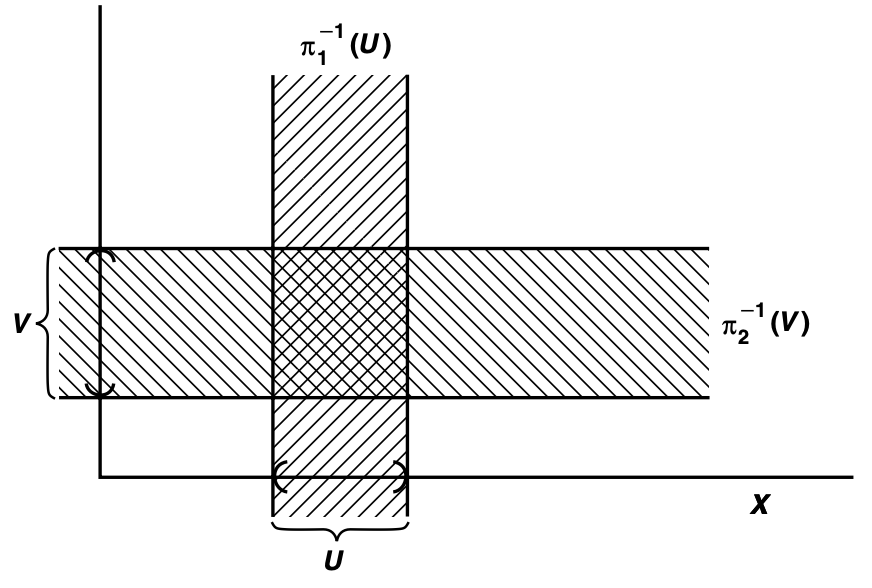
\includegraphics[width=0.8\textwidth]{/media/wu/file/stuuudy/notes/images/FiniteModelTheory/1.png}
\end{figure}

Let \(I_j\) be the set of partial isomorphism from \(\cala_l|\tau\) to \(\cala_k|\tau\) as
introduced in the preceding example. We have \((I_j)_{i\le m}:\cala_l|\tau\cong_m\cala_k|\tau\).
For \(j\ge2\) any \(p\in I_j\) preserves \(E\) too, that is,
\(I_j\subseteq\Part(\cala_l,\cala_k)\). If \(E^{A_l}ab\) for some \(a,b\in A_l\). Then
\(d_j(a,b)=4\) or \(\infty\) (since \(l\ge2^m\)). We need to ensure \(4<2^j\) and this is
why \(j\ge2\) (guess we loose the condition of the definition-.-). If \(d_j(a,b)=4\) then
clearly \(E^{A_k}p(a)p(b)\). If \(d_j(a,b)=\infty\), a big gap: how to prove \(E^{A_k}p(a)p(b)\) \label{Problem2}


Hence \((I_{j+2})_{j\le m-2}:\cala_l\cong_{m-2}\cala_k\)
and we have

the class of finite connected ordered graphs is not first-order axiomatizable
\end{examplle}

\begin{examplle}[]
For \(l\ge1\), let \(\calg_l\) be the graph given by a cycle of length \(l+1\). To be precise,
set
\begin{equation*}
G_l:=\{0,\dots,l\},\dots
E^{G_l}:=\{(i,i+1)|i<l\}\cup\{(i+1,i)|i<l\}\cup\{(0,l),(l,0)\}
\end{equation*}
Thus for \(l,k\in\N\), the disjoint union \(\calg_1\dot\cup\calg_k\) consists of a cyle of length
\(l+1\) and of a cycle of length \(k+1\). We show
\begin{equation*}
\text{if }l,k\ge2^m\text{ then }\calg_l\cong_m\calg_k\text{ and }\calg_l\cong_m
\calg_l\dot\cup\calg_l
\end{equation*}
In fact, for \(j\in\N\), define the distance \(d_j\) on a graph \(\calg\) by
\begin{equation*}
d_j(a,a')=
\begin{cases}
d(a,b)&\text{if }d(a,b)<2^{j+1}\\
\infty
\end{cases}
\end{equation*}
We verifies \((I_j)_{j\le m}:\calg_l\cong_m\calg_l\dot\cup\calg_l\) where
\(I_j\) is the set of \(p\in\Part(\calg_l,\calg\dot\cup\calg_l)\) with
\begin{equation*}
\norm{\dom(p)}\le m-j \quad\text{ and }\quad
d_j(a,b)=d_j(p(a),p(b))\text{ for }a,b\in\dom(p)
\end{equation*}
Condition \(d(a,b)<2^{j+1}\) is only to ensure \(\{(\min^A,\min^B),(\max^A,\max^B)\}\in I_j\) for
every \(j\le m\) as \(l,k\ge 2^m\). 

For every \(j<m\), \(p\in I_{j+1}\) and \(a\in G_l\), if there is a \(a'\in\dom(p)\)
s.t. \(d_j(a,a')<2^{j+1}\) then there is a unique \(b\) for which \(q=p\cup\{a,b\}\) is a partial
isomorphism. Else, let \(\dom(p)=\{a_1,\dots,a_r\}\). Assume \(a_i<a<a_{i+1}\) (abuse of notation
of course)




We note two consequents.
\begin{itemize}
\item The class CONN of connected finite graphs is not axiomatizable in first-order logic
\end{itemize}


   \begin{equation*}
\calg_{2^m}\in\text{CONN}, \calg_{2^m}\dot\cup\calg_{2^m}\not\in\text{CONN},
\calg_{2^m}\equiv_m\calg_{2^m}\dot\cup\calg_{2^m}
   \end{equation*}

\begin{itemize}
\item The global relation TC , the relation of transitive closure on the class GRAPH of finite
graphs, is not first-order definable
\end{itemize}


Suppose \(\psi(x,y)\) is a first-order formula defining TC on GRAPH. Then CONN would be the class of
finite models of \(\forall x \forall y(\neg x=y \to \psi(x,y))\)
\end{examplle}

\begin{exercise}
\label{ex2.3.9}
Set \(\tau=\{E\}\). For \(l\ge1\) let \(\calb_l\) and \(\cald_l\) be the \(\tau\)-structures
given by
   \begin{align*}
&B_l:=\{0,\dots,l\},\quad E^{B_l}:=\{(i,i+1)|i<l\}\\
&D_l:=\{0,\dots,l\},\quad E^{D_l}:=\{(i,i+1)|i<l\}\cup\{(l,0)\}
   \end{align*}
Given \(m\ge0\), show that \(\calb_l\cong_m\calb_l\dot\cup\cald_l\) for sufficiently large \(l\).
Conclude that the class of finite acyclic digraphs is not axiomatizable in first-order logic
\end{exercise}

\begin{proof}

\end{proof}

\begin{proposition}[]
The product, the disjoint union and the ordered sum preserve \(\equiv_m\)
\end{proposition}

\begin{proof}
Suppose \(\cala_1\equiv\calb_1\) and \(\cala_2\equiv_m\calb_2\). By Ehrenfeucht's Theorem there
are winning strategies for the duplicator in the games \(G_m(\cala_1,\calb_1)\)
and \(G_m(\cala_2,\calb_2)\). We refer to these strategies as \(S_1\) and \(S_2\)
\begin{enumerate}
\item \(G_m(\cala_1\times\cala_2,\calb_1\times\calb_2)\): we simultaneously play games
in \(G_m(\cala_1,\calb_1)\) and \(G_m(\cala_2,\calb_2)\).
\end{enumerate}
\end{proof}

\begin{corollary}[]
\begin{enumerate}
\item If \((\cala_1,\bara_1)\equiv_m(\calb_1,\barb_1)\)
and \((\cala_2,\bara_2)\equiv_m(\calb_2,\barb_2)\) then
\((\cala_1\dot\cup\cala_2,\bara_1,\bara_2)\equiv_m(\calb_1\dot\cup\calb_2,\barb_1,\barb_2)\)
\item If \((\cala_1,\bara_1)\equiv_m(\calb_1,\barb_1)\)
and \((\cala_2,\bara_2)\equiv_m(\calb_2,\barb_2)\) then
\((\cala_1\lhd\cala_2,\bara_1,\bara_2)\equiv_m(\calb_1\lhd\calb_2,\barb_1,\barb_2)\)
\end{enumerate}
\end{corollary}


\subsection{Hanf's Theorem}
\label{sec:org15f9460}
All vocabularies in this and the next section will be relational unless stated otherwise. For a
nonempty subset \(M\) of a structure \(\cala\) we denote by \(\calm\) the substructure
of \(\cala\) with universe \(M\)

Given a structure \(\cala\), we define the binary relation \(E^A\) on \(A\) by
   \begin{align*}
E^A:=\{(a,b)|a\neqb,\text{ and }&\text{there are $R$ in $\tau$ and $\barc$ s.t. }R^A\barc\\
&\text{and $a$ and $b$ are components of the tuple }\barc\}
   \end{align*}
\section{Problem List}
\label{sec:org28ebcb9}
\ref{Problem1}

\ref{Problem2}
\end{document}